To look at the energy consumption in detail, a power analyser was used as the power supply.
To carry out measurements, the ADP5090 with the solar cells and super cap was disconnected and the remaining components connected to the power analyser with a fixed voltage of 3.3\,V.
This way, the voltage and current could be over one write-cycle could be tracked.
The result is plotted in Figure \ref{results:ui}.
\begin{figure}[ht]
	\centering
	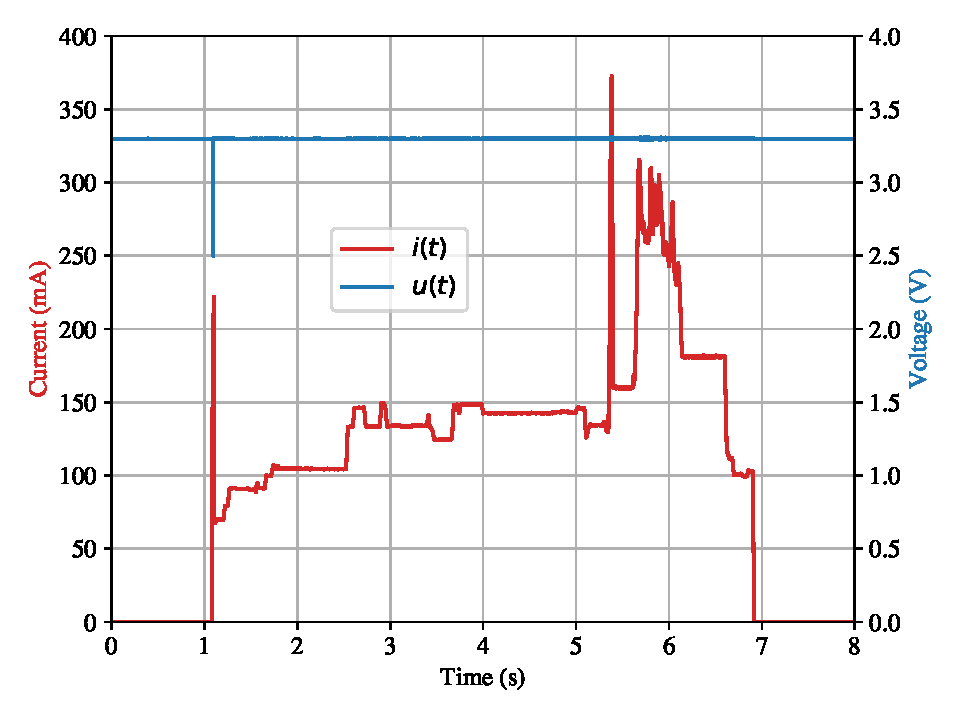
\includegraphics[width=0.9\textwidth]{5-results/energy/logger/ui.pdf}
	\caption{Current and Voltage during one write-cycle.\label{results:ui}}
\end{figure}
One write-cycle takes approximately 5.8 seconds.
In this interval, the STM32, nRF52480 and display driver are active.
Clearly visible is the inrush current peak.




\begin{figure}[ht]
	\centering
	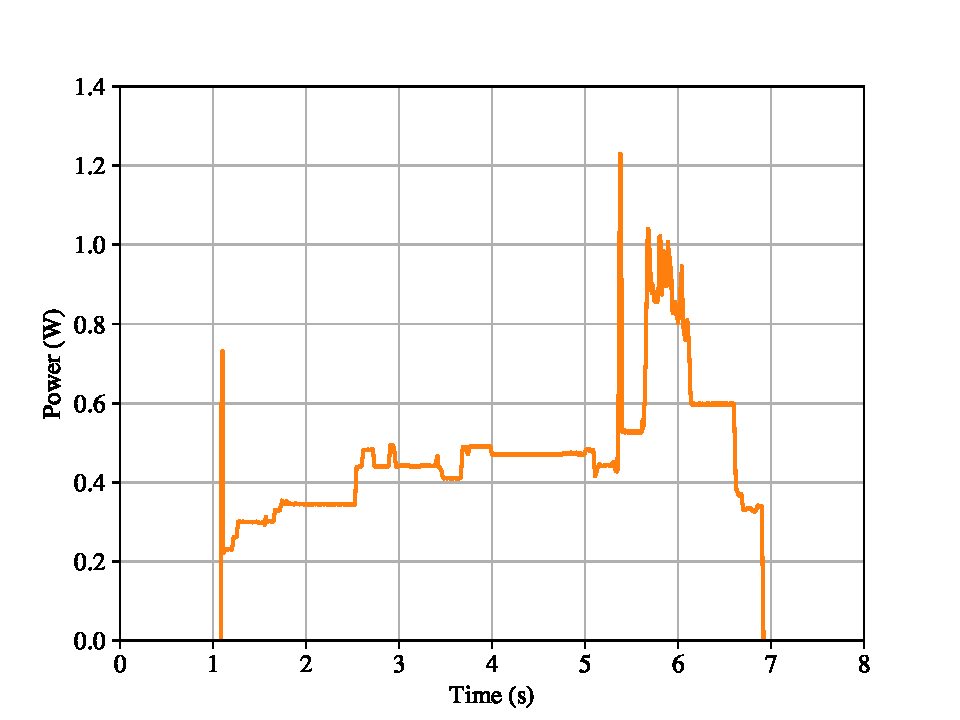
\includegraphics[width=0.9\textwidth]{5-results/energy/logger/p.pdf}
	\caption{Power consumption during one write cycle.\label{results:p}}
\end{figure}